\documentclass[11pt]{article}

%\input strowpreprint
%\usepackage{helvet}
\usepackage[T1]{fontenc}
\usepackage[expert]{lucidabr}
\usepackage{graphicx}
\usepackage{sidecap}
%\usepackage{floatrow}
\usepackage[usenames]{color}
\usepackage{epstopdf}
\usepackage{amsmath}
\usepackage[margin=5pt,font=footnotesize,labelfont=bf,textfont=md]{caption}
\usepackage{wrapfig}

\newcommand{\kc}{\textsf{kCARTA}\xspace}
\newcommand{\sa}{\textsf{SARTA}\xspace}
\newcommand{\sasc}{\textsf{SARTA-CLOUDY}\xspace}
\newcommand{\pcrtm}{\textsf{PCRTM}\xspace}

% figure1 figure1-caption figure1-label figure2 figure2-caption figure2-label
\newcommand{\dfigure}[6]
{
\begin{figure}
  \begin{minipage}[t]{0.45\textwidth}
  \centering
  \includegraphics[width = 1.00\textwidth]{#1}
   \caption{#2}  \label{#3}
  \end{minipage}
  \hfil
  \begin{minipage}[t]{0.45\linewidth}
  \centering
  \includegraphics[width = 1.00\textwidth]{#4}
   \caption{#5}  \label{#6}
  \end{minipage}
\end{figure}
}

\usepackage{xspace}
\newcommand{\wn}{cm$^{-1}$\xspace}
\newcommand{\um}{$\mu m$\xspace}
\newcommand{\cd}{CO$_2$\xspace}
\newcommand{\water}{H$_2$O\xspace}
\newcommand{\methane}{CH$_4$\xspace}
\newcommand{\nitrogen}{N$_2$\xspace}
\newcommand{\nitrous}{N$_2$O\xspace}
\newcommand{\oxygen}{O$_2$\xspace}
\newcommand{\ozone}{O$_3$\xspace}
\newcommand{\mydeg}{\mbox{$^\circ$}}

%---------------------------------------------------------------------------
\makeatletter
\renewcommand{\section}{\@startsection {section}{1}{\z@}%
                                   {-3.5ex \@plus -1ex \@minus -.2ex}%
                                   {2.3ex \@plus.2ex}%
                                   {\reset@font\large\bfseries}}
\renewcommand{\subsection}{\@startsection{subsection}{2}{\z@}%
                                     {-3.25ex\@plus -1ex \@minus -.2ex}%
                                     {1.5ex \@plus .2ex}%
                                     {\reset@font\normalsize\bfseries}}
\makeatother
%---------------------------------------------------------------------------
% Indent captions a little
%\setlength{\captionmargin}{10pt}
\parindent=1.2em
\parskip=0.5ex

%  For the tables
\def\tstrut{\vrule height 2.5ex depth 1.2ex width 0pt}
\def\tstruta{\vrule height 0ex depth 1.2ex width 0pt}
%---------------------------------------------------------------------------
% If use fancyhdr
% \lhead{}
% \rhead{}
% \chead{}
% \lfoot{\small\sf Page \thepage\ of \pageref{LastPage}}
% \rfoot{\small\sf L. Strow/UMBC}
% \cfoot{\small\sf AIRS and IASI Intercal}
%\renewcommand{\headrulewidth}{0pt}  % only with fancyhdr
%\pagestyle{plain}
\usepackage{geometry}
\geometry{letterpaper,margin=1.0in,vcentering}


%\lhead{\textsf{\textbf{DRAFT}}}

\title{\textsf{SARTA CLOUDY}: A Fast Forward Model Version of
  \textsf{SARTA}\\ with Cloud/Aerosol Scattering}

\author{S. De Souza-Machado, L. L. Strow, S. E. Hannon \\
      University of Maryland Baltimore County, Baltimore, MD 21250 USA}

\begin{document}

\maketitle

\begin{abstract}

The \textsf{SARTA CLOUDY} code is a modification of the UMBC clear sky \textsf{SARTA} code, allowing users to compute 
synthetic infrared radiances for the AIRS instrument, in the presence of clouds and aerosols. By re-parameterizing the
cloud scattering parameters into effective optical depths, the effect of clouds on upwelling radiation from
the Earth's atmosphere is effectively recast as that of (an) additional absorbing gas(es), which allows us to use 
the efficient radiative transfer algorithm of the clear sky code. The liens of the code are that model vertical cloud
fields (from eg ECMWF) need to be reshaped into at most two slab clouds. However, comparisons against packages 
which uses sophisticated algorithms (eg maximal overlap clouds and scattering trained on DISORT algorithm) shows that
the \textsf{SARTA CLOUDY} code produces radiances accurate to about 3K (converted to equivalent Brightness Temperature)

\end{abstract}

\section{Introduction}

This document gives an overview of \sasc, which is a Fast Infrared Atmospheric Radiative Transfer algorithm,
written to simply but accurately account for the effects of scattering by aerosols and clouds. This scattering package is 
directly based on our clear sky fast algorithm \sa, and so should be relatively straightforward for users familiar with 
the clear sky version, to integrate and use. In addition, the code is based on treating the effects of cloud and aerosols 
as that of additional absorptive gases, which means the radiative transfer retains its speed and efficiency. 

We begin by outlining the clear sky monochromatic algorithm, followed by a discussion of the scattering model we
chose to use for the monchromatic case. We then follow with a brief discussion of the challenges in making a code
for polychromatic clear sky transfer, and how the scattering algorithm can be easily adapted to work in this
polychromatic case as well.

We have already successfully used the scattering code to retrieve dust loadings and heights, for individual AIRS 
Fields-of-Views \cite{mac:10}. Assuming we knew the height of the dust layer, using a handful of AIRS channels, 
three iterations for convergence were done in a matter of milliseconds, for each AIRS pixel. We envision a similar approach 
for an operational retrieval, which we discuss. A discussion of how we implement Numerical Weather Prediction model 
fields for use with our algorithm then follows. 

We then show comparisons of window channel radiances computed using ECMWF/ERA fields, versus actual AIRS observations. Finally
we show comparisons of radiances produced by \sasc versus those produced by a more sophisticated algorithm, and argue that
for operational retrieval of temperature and humidity, the accuracy of our code is more than sufficient.

\section{Monochromatic Clear sky Radiative transfer algorithm}

As a monochromatic beam of radiation propagates through a layer, the change in diffuse beam
intensity $R(\nu)$ in a plane parallel medium is given by the standard
Schwartschild equation \cite{lio:80,goo:89,edw:92}

\begin{equation}
\mu \frac{dR(\nu)}{dk_{e}} = -R(\nu) + J(\nu)
\label{eqn:sch}
\end{equation}

where $\mu$ is the cosine of the viewing angle, $k_{e}$ is the extinction
optical depth, $\nu$ is the wavenumber and $J(\nu)$ is the source function. For
a nonscattering ``clear sky'', the source function is usually the Planck
emission $B(\nu,T)$ at the layer temperature $T$, leading to an equation that
can easily be solved for an individual layer. Dividing the atmosphere into
layers and propagating the solution through the layers, the final upwelling radiance
(for a downlooking instrument) can be written in terms of four components :

\begin{equation}
R(\nu) = R_{s}(\nu) + R_{\text{layer emission}}(\nu) + R_{th}(\nu) + R_{solar}(\nu)
\label{eqn:sch_detail}
\end{equation}

which are the surface, layer emissions, downward thermal and solar terms
respectively. The terms in the equation are relatively straightforward, and the resulting algorithm is 
usually quite efficient. 

\begin{wrapfigure}{l}{0.45\textwidth}
\centering
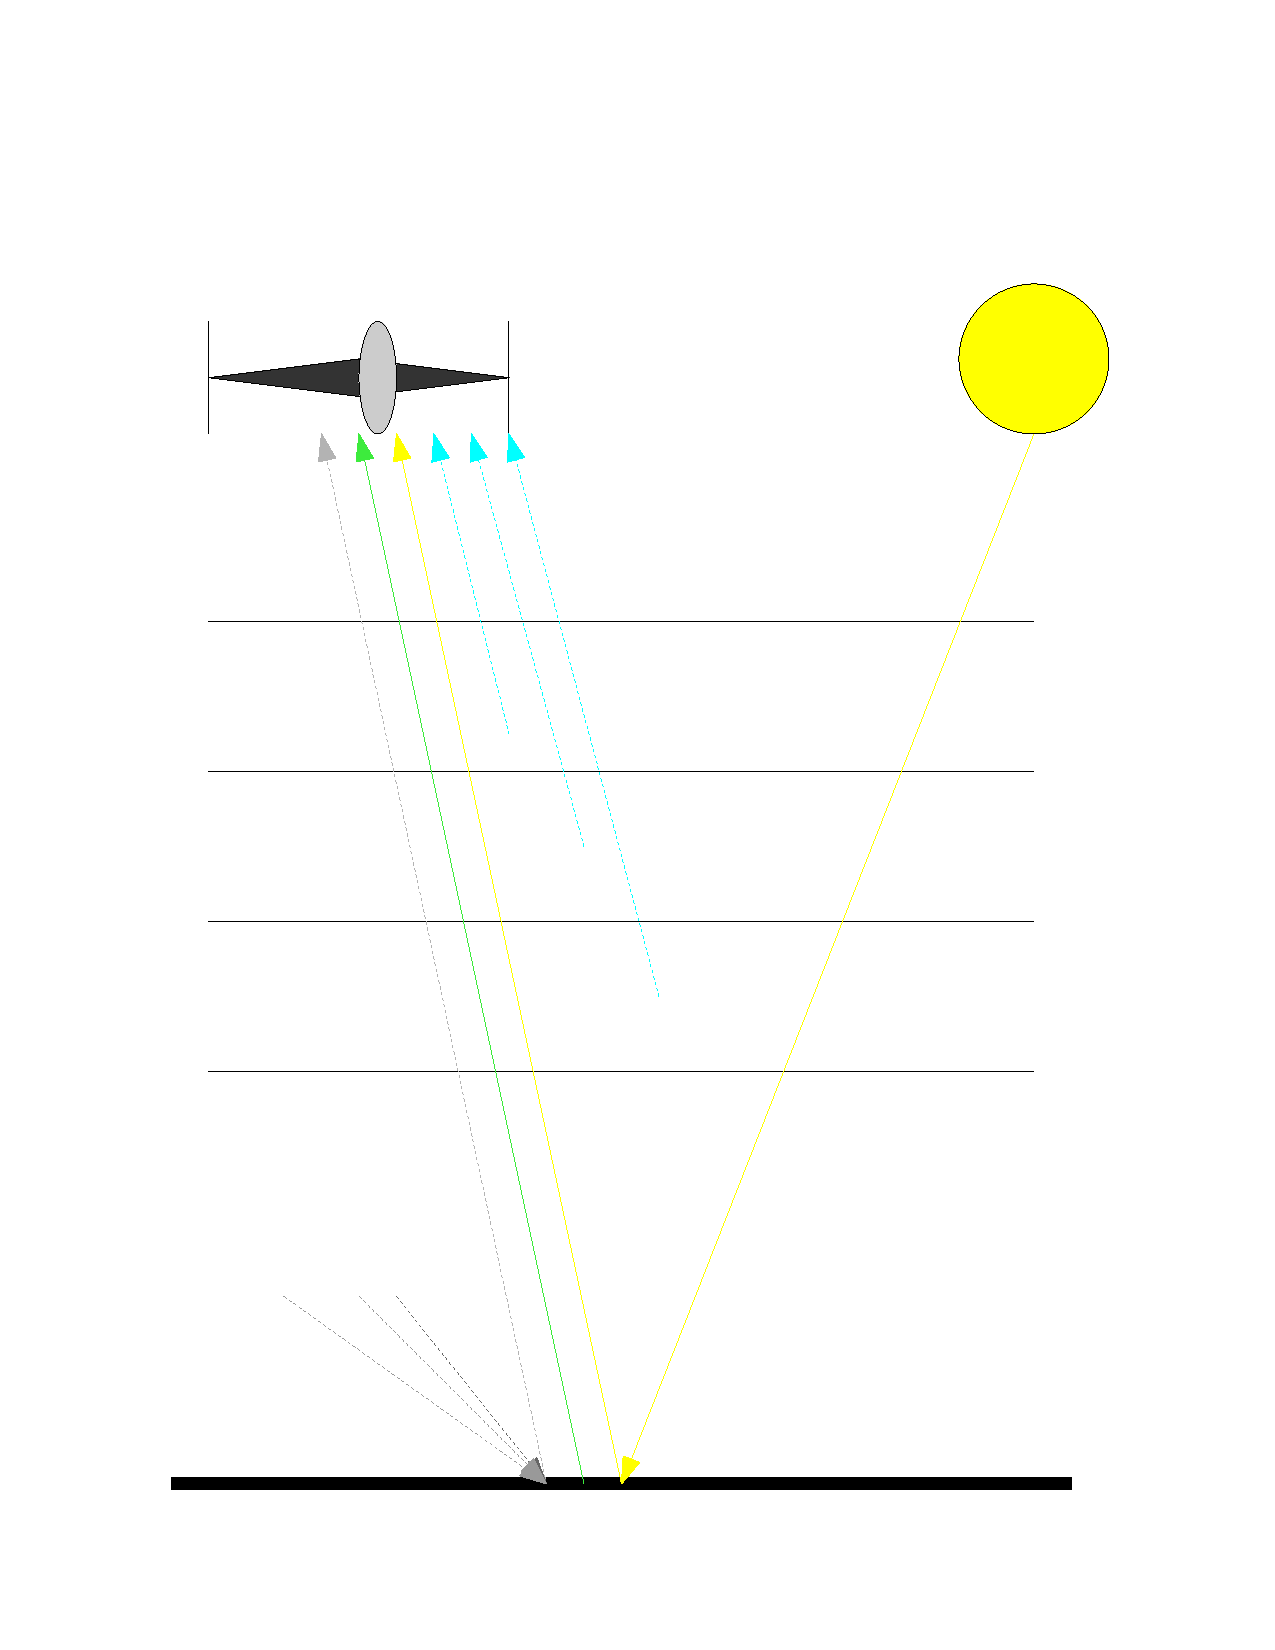
\includegraphics[width=0.45\textwidth]{Figs/radiation1.pdf}
\caption{Illustration of contributions to measured Top Of Atmosphere radiance :
 (blue) layer emission, (green) surface, (yellow) solar and (gray) background thermal}
\end{wrapfigure}
Our monochromatic code \kc indexes the atmosphere so that layer $1$ is the bottom and
$N$ (=100) the uppermost. Denoting $B(T)$ as the Planck function, $T_{s}$ as
the skin surface temperature, $\epsilon_{s}$ as the surface emissivity,
$\theta$ as the satellite viewing angle, $\theta_{solar}$ as the sun zenith
angle, $\tau_{i}(\nu)$ as the transmission of layer $j$
($\tau_{i}(\nu) = exp^{-k_{i}(\nu)}$), $\tau_{j \rightarrow m}(\nu)$ as the
transmission from layer $i$ to layer $m$, the individual terms are computed in
monochromatic codes, such as \kc as follows.
\subsection{Surface emission}

This is simply the emission from the surface (temperature $T_{s}$),
multiplied by the surface emissivity $\epsilon_{s}$ to account for the surface
not being a perfect black body, and attenuated by absorption due to the
atmosphere.

\begin{eqnarray*}
R_{s}(\nu) & = & \epsilon_{s} B(\nu,T_{s}) \tau_{1 \rightarrow N}(\nu,\theta)
\end{eqnarray*}

\subsection{Layer emission}

As the radiation emitted from the surface propagates up, it is absorbed by
the layer of gas above it, and then re-emitted. This atmospheric emission
happens layer by layer :
\begin{eqnarray*}
R_{layer emission}(\nu) & = & \sum_{i=1}^{i=N} B(\nu,T_{i})
(1.0 - \tau_{i}(\nu)) \tau_{i+1 \rightarrow N}(\nu,\theta))
\end{eqnarray*}

Layers with negligible absorption ($\tau_{i} \rightarrow 1$) contribute
negligibly to the overall radiance, while those with large optical depths
 ($\tau_{i} \rightarrow 0$) ``black'' out radiation from below.
$(1.0 - \tau_{i}(\nu))$ is the emissivity of the layer while
$(1.0 - \tau_{i}(\nu)) \tau_{i+1 \rightarrow N}(\nu,\theta))$ is the weighting
function $W_{i}$ of the layer.

\subsection{Background thermal radiation}

The atmosphere also emits radiation downward in a manner analogous to the
upward layer emission just discussed. Upon reaching the surface, this
radiance may be reflected upward. At the surface, the magnitude of this
background term is :

\begin{eqnarray}
R_{th}^{surface}(\nu) & = & \sum_{i=N}^{i=1}
\int_{0}^{2\pi}d\phi
\int_{0}^{\pi/2} d(cos\theta) cos\theta \rho(\theta,\phi)
\times B(\nu,T_{i}) \times \Delta \tau
\label{bckgnd_eqn}
\end{eqnarray}

\noindent Here $ \Delta \tau = (\tau_{i-1 \rightarrow ground}(\nu,\theta)-
 \tau_{i \rightarrow ground}(\nu,\theta))$.
Note the summation has been reversed, as we start out from the top of the
atmosphere $N$, and come down to ground $i=1$.
This background thermal term also depends on the surface reflectivity $\rho$.
If one assumes that the reflectivity of the surface is Lambertian, then $\rho$
can be rewritten as $\frac{1 - \epsilon_{s}}{\pi}$. This entire background
reflected term is negligible in regions that are ``blacked out,'' but in
the window regions can contribute as much as 0.5 K of the total radiance when
reflected back up to the top of the atmosphere.

Equation \ref{bckgnd_eqn} involves an angular integration that needs to
be done quickly but accurately. Layer by layer, the
Mean Value Theorem means Eq. \ref{bckgnd_eqn} can be rewritten in terms of an
effective diffusive angle $\theta^{i}_{d}$ at each layer $i$ :
\begin{eqnarray*}
R_{th}^{surface}(\nu) & =
                 & \frac{1 - \epsilon_{s}}{\pi} \frac{1}{2} \sum_{i=N}^{i=1}
B(T_{i}) \left[ \tau_{i-1 \rightarrow ground}
(\nu,\theta^{i}_{d1})-\tau_{i \rightarrow ground}(\nu,\theta^{i}_{d2}) \right]
\end{eqnarray*}
where based on the layer to ground transmissions of the $i,i-1$ $th$
layers,  $\theta^{i}_{d1},\theta^{i}_{d2}$ are the optimum diffusion angles.

The value of $\theta^{i}_{d}$ that is often used is that of $\arccos(3/5)$
\cite{lio:80}, especially for low optical depths ($k \le 1$).  A check of the
accuracy of using this angle at all layers against an accurate computation
using Eq. \ref{bckgnd_eqn}, showed that the errors in the window regions could
be larger than 0.2 K, and would be even larger over land surfaces where the
land surface emissivity is as low as 0.8. Instruments such as AIRS have
channel radiance accuracies better than 0.2K, making it important to compute
the background thermal correctly throughout the wavenumber region encompassed
by the spectroscopic \kc database.

As Eq. \ref{bckgnd_eqn} is computationally intensive, we devised the following.
In an optically deep region, the surface is blacked out and one need not
accurately compute the reflected term, and so $\arccos(3/5)$ can be used
at all layers.

Conversely in an ``optically thin'' region, the layers closest to the ground
contribute most to $R_{th}(\nu)$ (see discussion of weighting function above).
For each 25 \wn region, the layer $L$ above which $\arccos(3/5)$ can be
safely used, was determined. Below this layer, we use a lookup table where
$\theta^{i}_{d}$ angle is parameterized as a function of layer-to-ground
optical depth (and hence transmittance).

With surface emissivity set at 0.8, $L$ was chosen such that the brightness
temperature errors at the top of the atmosphere were less than 0.1K for the
sampling of profiles tested. The accuracy was checked by propagating the
thermal background between the top of the atmosphere and the ground using this
method, and comparing it to the results from using Eq. \ref{bckgnd_eqn}.

\subsection{Solar radiation}

Letting the solar reflectance be denoted by $\rho(\nu)$, then

\begin{eqnarray*}
R_{solar}(\nu) & = & \rho(\nu) B_{solar}(\nu) cos(\theta_{solar}) \times \\
& &                 \tau_{N \rightarrow ground}(\nu,\theta_{solar}))
                 \tau_{ground \rightarrow N}(\nu,\theta))
                 \Omega_{solar}
\end{eqnarray*}

$\rho$ is usually (inaccurately) modeled as
$\rho = \frac{1 - \epsilon_{s}}{\pi}$.
$\Omega_{solar} = \pi(r_{s}/d_{se})^{2}$ is the solid angle subtended at the
earth by the sun, where $r_{e}$ is the radius of the sun and $d_{se}$ is the
earth-sun distance. The solar radiation incident at the TOA $B_{solar}(\nu)$
comes from datafiles, and is modulated by the angle the sun makes with the
vertical, $cos(\theta_{solar})$.

\subsection{\textsf{Monochromatic PCLSAM} scattering algorithm}
\kc can be interfaced with advanced scattering codes such as DISORT \cite{stam:88}
and RTPSEC \cite{dee:98}. While well tested and numerically very accurate, these codes are
complicated, leading to run times that can be significantly longer than for the clear sky case.
In addition, the separation of radiative effects into solar and terrestrial means, 
for typical infrared instruments such as AIRS, IASI and CRiS, means one can optimize 
codes to work on either the thermal and/or the short wave infrared regions. 

We chose to implement a fast code optimized to work where scattering is
less important than absorption effects. In the thermal infrared, the effects of
scattering due to aerosols and clouds is less than the effects of absorption, making
the \textsf{PCLSAM} (Parameterization of Cloud Longwave Scattering for use in
Atmospheric Models) scheme \cite{cho:99} very attractive. Since the model assumes 
the downward intensity through a cloud layer is the same as the Planck emission at the
cloud temperature and thus simplifies the problem, it typically slightly
overestimates the final TOA radiance. This algorithm changes the optical
depth from $k$ to a parameterized number $k\prime$ as described briefly
below; more details can be found in \cite{cho:99,mat:05}.

For each layer $i$ that contains scatterers, we replace the optical depth with
the total optical depth
   $k_{total}(\nu) = k_{atm}^{gases}(\nu) + k^{scatterer}_{extinction}(\nu)$.
However this is reparameterized as
\[
k\prime(\nu) = k_{total}(\nu) \times \{ (1-\omega(\nu) (1-b(\nu)) \}
\]

where the effective single scattering albedo $\omega$ and backscatter $b$ are
obtained from the scatterer-only case $\omega_{0}$ using
\[
\omega(\nu) = \omega_{0}(\nu) k^{scatterer}_{extinction}(\nu)/k_{total}(\nu)
\]
\[
b(\nu)      = (1 - g(\nu))/2
\]

Note that if there are no scatterers in the layer, $\omega(\nu) \rightarrow 0$ and
we recover the clear sky optical depth. 

This same parameterization of the optical depth can be repeated for all the
layers which contain scatterers, from which the radiative transfer algorithm
can be written in the same form as that for clear sky radiative transfer, with
very little speed penalty. Since
the scattering parameters $k^{scatterer}_{extinction},\omega_{0},g$ are stored
in lookup
tables as a function of particle size, it is trivial to obtain the derivatives
with respect to size and particle amount. This method therefore immediately
lends itself to be extended to compute scattering jacobians as well as fluxes,
in a manner exactly analogous to that for clear sky jacobians and fluxes.

We have attempted to account for solar scattering in the SWIR, but comparing to 
DISORT and actual AIRS observations, we state this a significant lien on the code
in this spectral region.
We note that while computing the direct beam scattered solar contribution, we
use the extinction optical depth $k$ in
  $ \left[ 1 - e^{-k (\frac{1}{\mu} + \frac{1}{\mu_{sun}})} \right]$, rather
than the parameterized optical depth $k \prime$.

Some points to note are that
\begin{itemize}
  \item While absorption spectra due to atmospheric gases has much structure, the crystal
        bonding, and smoothing over particle size distributions, "blurs" out sharp features, resulting 
        in smooth absorption and scattering parameters.
  \item Aerosol particles range in size from 0.1 um (smoke) to 4 um (dust) in diameter, which means 
        the thermal infrared is typically much more sensitive to dust than to smoke.
  \item Even for dust, non-sphericity of these particles is not a very big issue in the TIR.
        As long as realistic refractive indices are used, the results of Mie codes, integrated over 
        realistic particle size distributions, should suffice to produce scattering parameters that can be
        relied upon.
  \item Similarly water clouds can be assumed to be spherical, typically 20 um in diameter.
  \item Cirrus can come in many different types of shapes or "habits", which typically
        depend on temperature through the height of the cloud. Since the resulting ice 
        crystals can be quite large, whose shapes can deviate significantly from spherical, Mie codes should
        not be used to produce scattering parameters for use in terrestrial radiative transfer codes. 
        We use cirrus scattering parameters for ice aggregates or hexagonal plates, provided by
        Anthony Baran of the UKMO.
\end{itemize}

\section{SARTA Clear sky Radiative transfer algorithm}

Keeping the surface and layer emission terms, while ignoring the solar and background thermal terms, 
the monochromatic clear sky radiative transfer algorithm can be written as

\begin{eqnarray*}
R_{toa}(\nu) & = & \epsilon_{s} B(\nu,T_{s}) \tau_{1 \rightarrow N}(\nu,\theta) + \\
             &   &  \sum_{i=1}^{i=N} B(\nu,T_{i})
                   (1.0 - \tau_{i}(\nu)) \tau_{i+1 \rightarrow N}(\nu,\theta)) \\
             & = & \epsilon_{s} B(\nu,T_{s}) \mathcal{T}(\nu,\theta)^{1 \rightarrow N} + \\
             &   &  \sum_{i=1}^{i=N} B(\nu,T_{i}) \{ \mathcal{T}(\nu,\theta)^{i+1\rightarrow N} - 
                                                     \mathcal{T}(\nu,\theta)^{i \rightarrow N} \}
\end{eqnarray*}

from which the top-of-Atmosphere radiance for an AIRS channel would be given by
\begin{eqnarray*}
  R_{AIRS}(j) = \int_{\delta \nu_{j}} R_{toa}(\nu) SRF_{j}(\nu) d\nu
\end{eqnarray*}

Notice that in both the surface term and the atmospheric emission term, we deal with layer to 
space transmittances, which means we need to take into consideration what is above each layer during 
the iteration of the radiative transfer algorithm. For a monochromatic code, this is not an issue, as 
Beer's law applies.

On a 2.3 GHz machine, a \kc run from 605-2830 \wn would take about 90 seconds, as optical depths have to be 
generated for about 900000 wavenumber points (spanning the above interval at 0.0025 \wn spacing) for each 
of the 100 layers. The spectral convolution for all 2378 channels using Matlab would add on an additional 
$\sim$ 10 seconds to generate one synthetic AIRS clear sky spectrum with the \kc line-by-line code.

With AIRS providing about 3 million spectra per day, it would clearly be next to impossible to use \kc 
in its current guise, to analyze the data. A fast Stand Alone Radiative Transfer Model (SARTA) was written,
which 
takes a fraction of the above time (about 0.1 seconds) to generate one synthetic spectrum. For each AIRS
channel, a simplified view of how this this code works is as follows. The atmospheric gas absorption for  
\begin{wrapfigure}{l}{0.45\textwidth}
\centering
%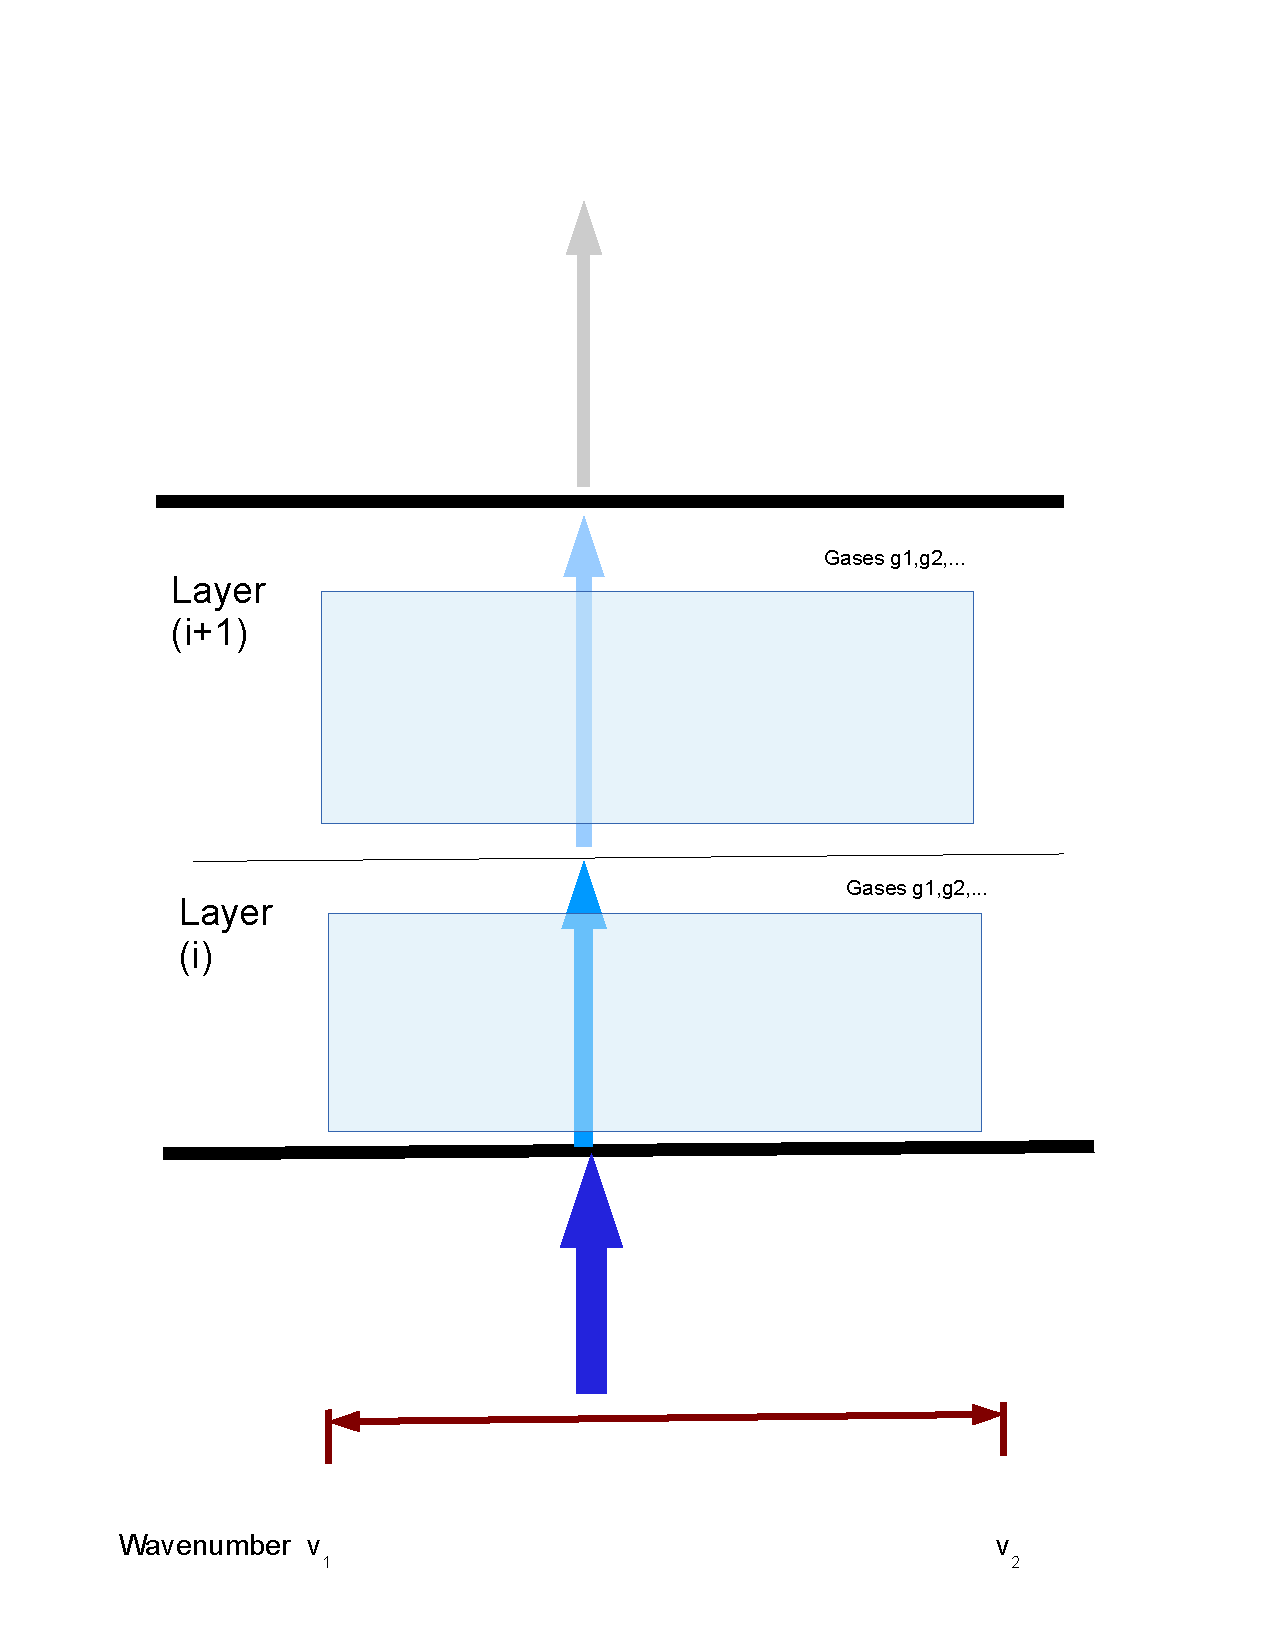
\includegraphics[width=1\textwidth,height=0.5\textheight]{Figs/twolayers.pdf}
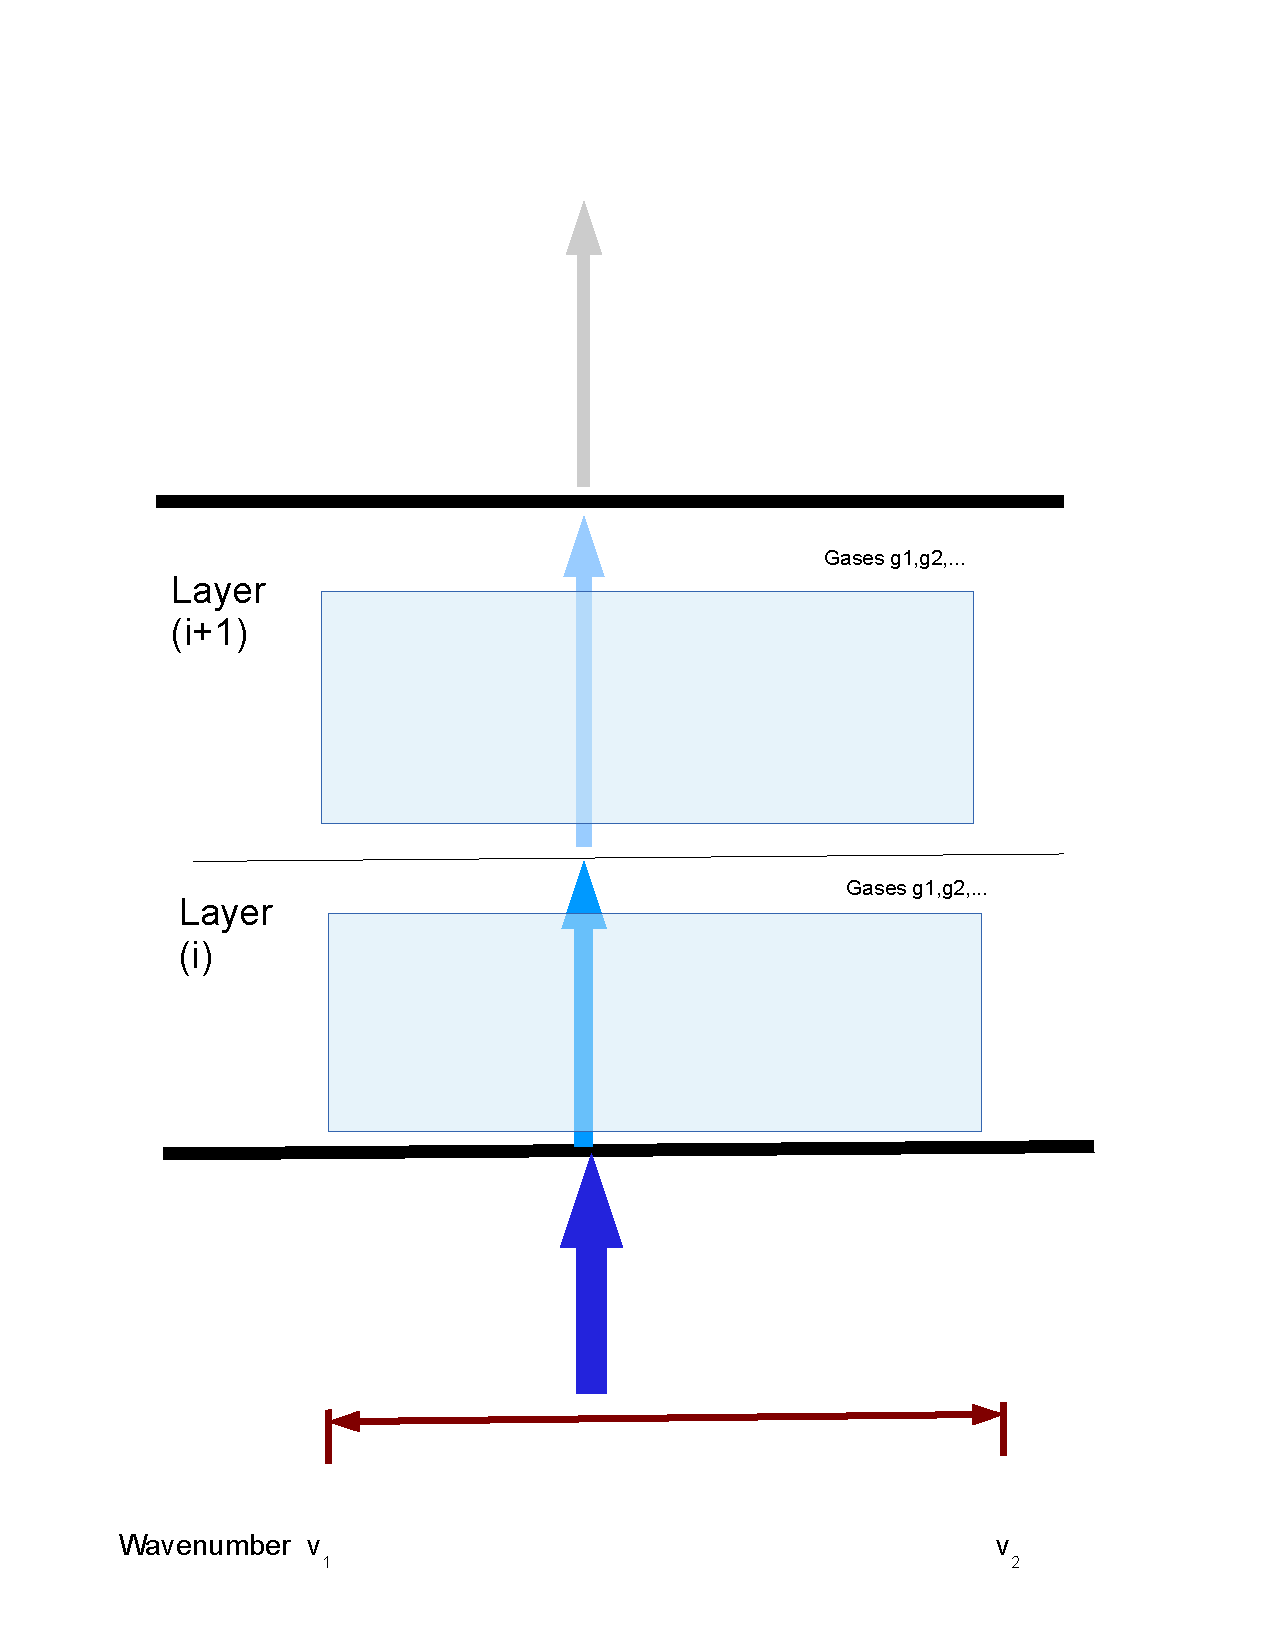
\includegraphics[width=0.45\textwidth]{Figs/twolayers.pdf}
\caption{
Pitfalls when applying Beer's law to finite width channels. Not only does it breakdown going from one layer to 
another, but in addition you cannot simply multiply in the contributions due to different gases
}
\end{wrapfigure}
each layer of the channel in question is parameterized in terms of predictors such as layer temperature, 
gas absorber amounts (separated into water vapor, ozone, other gases) and viewing angle geometry. A significant
complication arises since we are dealing with layer to space transmittances, coupled with convolutions over
finite channel widths. This leads to a breakdown in Beer's law. In other words, for example for two 
consecutive layers, if the monochromatic optical depth of each is $k(\nu))$ then, the transmittance from the 
bottom of one layer to the top of the next, is given monochromatically by
\begin{eqnarray*}
  \tau_{\nu}^{i \rightarrow i+1} & = & exp(-k_{i}(\nu)) \;\; exp(-k_{i+1}(\nu)) \\
\end{eqnarray*}
In other words, at each wavenumber, the total transmittance through both layers, is the product of the 
transmittances through each layer
\begin{eqnarray*}
  \mathcal{T}(\nu)^{i \rightarrow i+1}           & = &  \mathcal{T}(\nu)^{i} \;\;  \mathcal{T}(\nu)^{i+1}\\
\end{eqnarray*}
where $\mathcal{T}(\nu)^{l}$ is the monochromatic transmittance through layer $l$. 

However, this law breaks down when looking at the convolved transmittance. For example, for AIRS channel $j$,
\begin{eqnarray*}
  \tau_{airs}^{i \rightarrow i+1}(j) = \int_{\delta \nu_{j}} exp(-k_{i}(\nu)) \;\; exp(-k_{i+1}(\nu)) SRF_{j}(\nu) d\nu
\end{eqnarray*}
which is $NOT$ equal to 
\begin{eqnarray*}
  \int_{\delta \nu_{j}} exp(-k_{i}(\nu)) SRF_{j}(\nu) d\nu \;\; \int_{\delta \nu_{j}} exp(-k_{i+1}(\nu)) SRF_{j}(\nu) d\nu
\end{eqnarray*}
ie 
\begin{eqnarray*}
\mathcal{T}_{airs}^{i \rightarrow i+1}(j) \ne  \mathcal{T}_{airs}^{i}(j) \;\; \mathcal{T}_{airs}^{i+1}(j)
\end{eqnarray*}

When accounting for the convolved layer to space transmittance, not only does one have to consider the individual layers,
but within each layer, the total optical depth is a sum over all contributing gases, further complicating matters. 
For example, for atmospheric layer $i$, the total monochromatic optical depth is due to a sum of contributions of all 
gases $g$ such that 
\[
k_i(\nu) = k_i^{g1}(\nu) + k_i^{g2}(\nu) + .... + k_i^{gG}(\nu)
\]
from which the transmittance is $\tau_{i}(\nu) = \Pi_{g=1}^G exp(-k_i^{g}(\nu))$. For AIRS channel $j$, the polychromatic 
transmittance required for a Fast Model is then $\mathcal{T}_{airs}^{i}(j) = \int_{\delta \nu_{j}}  \tau_{i}(\nu) d\nu$, 
and one immediately sees a breakdown of Beer's law within the individual layers!

In the making of a Fast Forward Model, monochromatic radiative transfer becomes polychromatic radiative transfer, and 
the above needs to be taken into consideration. This is especially so in the case when wants to be able to consider 
effects of individual variable gases such as ozone, water vapor, CO2 separate from the fixed gases. \sa handles this 
problem by parameterizing effective layer to space transmittances, and then converting 
them to equivalent optical depths for each layer. Further details are given in \cite{han:02*1,str:02*2}.
\begin{eqnarray*}
\mathcal{T}^{eff,i}_{airs}(j) & = & \mathcal{T}_{airs}^{i \rightarrow N}(j) / \mathcal{T}_{airs}^{i+1 \rightarrow N}(j) \\
\mathcal{OD}^{eff,i}_{airs}(j) & = & -ln\{\mathcal{T}^{eff,i}_{airs}(j) \}
\end{eqnarray*}

This means that for each layer $i$ and AIRS channel $j$, we have the effective optical depth due to atmospheric gases. 

\section{SARTA Cloudy/aerosol sky Radiative transfer algorithm}

Recall from the earlier discussion on monochromatic scattering radiative transfer, the effects of clouds and 
aerosols was included by simply 
adding in the effective scattering optical depth. For the polychromatic case, we simply add on the effects of the 
relevant scatterer, where needed, and then perform the radiative transfer using the clear sky algorithm. The only time 
penalty incurred for each cloud/aerosol contaminated column of air, is reading in and interpolating the relevant 
scattering tables. Since the scattering parameters vary smoothly in spectral frequency, it is very straightforward to 
construct scattering optical depth tables for the $j$th AIRS channel for scattering species $S$; then for an arbitrary 
loading $q(j,i)^{S}$ g/m2
 \begin{eqnarray*}
  extinction(j,i,r)^{S} & = &  extinction(r)^{S}(1) \times  q(j,i)^{S} \\
  ssa(j,i,r)^{S} & = &  ssa(r)^{S} \\
  g(j,i,r)^{S} & = &  g(r)^{S} \\
\end{eqnarray*}
where $ssa$ and $g$ are the single scattering albedo and asymmetry parameter respectively, and $extinction(j,r)^{S}(1)$ 
is the extinction for a column loading of 1 g/m2; the particle size is denoted by $r$. The effective optical depths for 
channel $j$, layer $i$ are then given by
\[
   k_{airs,total}^{j,i} = k_{airs}^{j,i}(gases) + extinction_{airs}^{j,i}(scatterer)
\]
However again, to account for scattering effects, this is reparameterized as
\[
k\prime_{airs}^{j,i} = k_{airs}^{j,i} \times \{ (1-\omega(j,i) (1-b(j,i)) \}
\]

where the effective single scattering albedo $\omega$ and backscatter $b$ are
obtained from the scatterer-only case $\omega_{0}$ using
\[
\omega(j,i) = ssa(j,i) \times extinction(j,i)/k_{airs,total}^{j,i}
\]
\[
b(j,i)      = (1 - g(j,i))/2
\]

after which the radiance at top of the atmosphere can be calculated using the standard equations of radiative transfer.

\section{Outline for AIRS L2 operational retrievals}

As mentioned earlier, we have already successfully used our code to retrieve dust loadings and heights, for a 
sandstorm which eventually blew over the Mediterranean in late February, 2007 \cite{mac:10}. The optical depth 
retrievals agreed with many A-Train sensors, including MODIS, PARASOL, OMI and Calipso. Out task was arguably made easier
by assuming the dust filled the Field-of-View, fixed particle size distribution, particle refractive index and 
effective particle size (4um diameter). One complication was to also solve for dust height, instead of using eg 
climatological heights. For testing purposes, 
if the current operational AIRS L1/L2 dust flag detects dust, and we assume fixed particle sizes and aerosol height
from climatology, we can almost always retrieve dust loadings that correlate very well with eg MODIS aerosol optical depths,
{\em even if they are not necessarily accurate because we potentially used an incorrect height}.

Wh have also prototyped a more complete L2 retrieval in the presence of dust. Again in this case, we made some assumptions
namely we know the effective particle size and height of the dust, and made a further assumption that we knew the underlying
surface emissivity (over ocean or land). With these a-priori assumptions, we were able to solve for $T(z),WV(z)$ and surface
temperature, as well as dust loading, using a 1D-var approach.

With the above experience, we outline some suggestions for including the \sasc code in an operation AIRS L2 retrieval.
The additional $a-priori$ parameters required would be similar to those we needed for the dust case, namely cloud fraction,
height, particle size and surface emissivity; in addition we would need cloud phase. The current L2 retrieval provides 
estimates of cloud heights and fractions, from which one could easily produce the required parameters. From the height(s) 
we could infer phase; given this phase information, one could assume 20 um effective particle sizes for water clouds, or use
the corresponding (climatological) temperature to infer cirrus particle size. So the AIRS L2 algorithm would then
only need to solve for two additional parameters (ice and water cloud loading), in addition to the usual $T(z),WV(z)$
and surface temperature estimates it provides. We hope that using \sasc will improve the yield of "good" AIRS 
retrievals, especially closer to the surface.

An expansion of this idea would be to account for the effects of dust, if its presence is indicated by the
AIRS L1 flag. Again, we would simply assume a fraction of 1, 4um effective size, and dust height from climatology; 
it may be more prudent to assume no cloud under or above the cloud for such cases. 

\section{Implementation details for NWP models}

Typically, Numerical Weather Prediction (NWP) models provide vertically resolved temperature and gas profiles at each 
grid point. Both \kc and \sa ingest integrated versions of these profiles (via the associated $klayers$ code), and use 
this information to compute optical depths which are then fed into the radiative transfer algorithm.

In addition, the NWP models also provide cloud fields at the same vertical resolution. When developing the \sasc code, we
quickly realized that although liquid water and cirrus profiles were provided, as were total cloud fractions, we would 
run into an infinity of problems implementing cloud fractions, and in particular overlapping cloud fractions, at each 
AIRS layer. For this reason, we limit the \sasc code to having cloud/aerosol in at most $two$ slabs. The input parameters
for each of these slabs $k=1,2$ 
 should include
\begin{itemize}
\item species (water cloud [101], ice (habit) cloud [201], or aerosol (type)[301])
\item particle effective size (in um)
\item loading (in g/m2); roughly for ice 50g/m2 = 1 OD, and for water 2g/m2 = 1 OD
\item cloud/aerosol top (mb)
\item cloud/aerosol bottom (mb)
\item cloud fraction $0 \le c(k) \le 1$
\end{itemize}

In addition, we need a combined cloud fraction $C(k,l)$. For channel $j$ the total radiance at the top of the atmosphere 
would then be
\[
R_{AIRS}(j) = (1 -  (c(1) + c(2) - C(1,2)) R_{clear}(j) + c(1) R^{(1)}_{cloud}(j) + c(2) R^{(2)}_{cloud}(j)
\]
where $R_{clear}(j)$ is the radiance for a clear column of air, and $R^{(k)}_{cloud}$ is the radiance assuming 
a column of atmosphere completely filled with cloud of type $k=1,2$. Obviously if $c(1) = c(2) = C(1,2) = 0$ we get 
back a clear sky radiance. Depending on $c(k),k=1,2$ this means at worst, the cloudy sky code is about 3 times 
slower than the clear sky code.

% One important point is what temperature the cloud is at, if it spans pressures (p1,p2) that is thicker than 
% one AIRS layer, \textcolor{red}{Need to look at the code!}

\subsection{Types of scatterers}
We currently have scattering tables for a number of species. The tables span the full range of 2378 AIRS channels and a 
range of particle sizes; hence the scattering parameters for an arbitrary effective particle size is obtained by an 
interpolation. In addition the tables are for a particle loading of 1 g/m2; as explained above the extinction values for 
an arbitrary loading are obtained by a simple multiplication.
\begin{itemize}
  \item aerosol (type 301)
    \begin{itemize}
      \item desert dust
      \item volcanic ash
      \item effective diameter typically ranges from 0.5 to 10 um
    \end{itemize}
  \item cirrus (type 201)
    \begin{itemize}
      \item hex plates
      \item aggregates
      \item effective diameter typically ranges from 10 to 200 um
    \end{itemize}
  \item water (type 101)
    \begin{itemize}
      \item effective diameter typically ranges from 15 to 25 um
    \end{itemize}
\end{itemize}

\subsection{Cloud levels $\rightarrow$ slabs}

As mentioned above, we need to go from $\simeq$ 90 levels of cloud profile information, to two slabs. Our 
"emcwf2sarta" matlab routine does the necessary manipulations, summarized below. 

\subsubsection{Input requirements}

As stated above, in addition to the usual temperature and trace gas profiles, we also need the following information 
from ECMWF/ERA
\begin{itemize}
  \item p.ciwc : 91xP           cloud ice profiles
  \item p.ciwc : 91xP           cloud ice profiles
  \item p.cc   : 91xP           cloud total fraction
\end{itemize}

\subsubsection{Smooth the input profiles}
\begin{itemize}
  \item Normalize cloud profile eg \\ \hspace{1in} $normalized_{ice} = ice_{profile}(:,ii)/max(ice_{profile}(:,ii))$ 
  \item Smooth normalized profile  \\ \hspace{1in} $normalized_{ice} \rightarrow normalized_{ice}^{smoothed}$ 
\end{itemize}

\subsubsection{Turn smoothed profile into slab profiles}
\begin{itemize}
  \item Find how many peaks are present in this normalized profile, and "width" of peaks. 
  \item The widths will help determine the cloud top and bottom
  \item Start combining peaks so that we have at most two peaks for ice cloud, and two peaks for water cloud
  \item Finally, combine so at most we have two slabs
\end{itemize}

\subsubsection{Determine effective particle sizes, cloud amounts and cloud fractions}
\begin{itemize}
  \item Cloud amount for each slab is then determined by converting the original ice/water cloud profile (in g/g) to 
        integrated g/m2,
  \item Effective particle size for water is set to 20 um $\pm$ random amount
  \item Effective particle size for cirrus is set according to the temperature of the cloudtop (again, $\pm$ a random amount). 
  \item Cloud fracs for each cloud, and the overlap, are randomly set (using the "cc" field), so that they satisfy 
    \begin{itemize}
      \item c(1) $\le$ 1, c(2) $\le$ 1
      \item c(1,2) $\le$ min(c(1),c(2))
      \item clear = 1 - (c(1)+c(2) - c(1,2))
      \item c(1) exclusively = c(1) - c(1,2)
      \item c(2) exclusively = c(2) - c(1,2)
    \end{itemize}
\end{itemize}

\subsubsection{Examples}
Figures 3-6 illustrate the results of our "emcwf2sarta" code. Blue and Red are the ECMWF 91 level 
water and ice profiles (in g/g) while cyan and magenta are the water and cirrus slabs we end up with.
The horizontal extent of the slabs are the integrated cloud profiles, converted to g/m2 and normalized by
a factor of 10000 for the plots. It is possible to tweak the "emcwf2sarta" code in the future. For example
we can move the cirrus cloud higher, if we want to reduce overall computed radiances.

\dfigure{Figs/clouds_profile10.eps}{}{}{Figs/clouds_profile100.eps}{}{}
\dfigure{Figs/clouds_profile1000.eps}{}{}{Figs/clouds_profile2000.eps}{}{}

%\section{Timings}

\section{Comparison to AIRS observations}

We have been able to make some comparisons of \sasc against AIRS observations, for the 10 years of data available 
to us. Figure \ref{AIRS_obs_July} is a gridded map showing daytime AIRS 1231 \wn observations (converted to BT),
while Figure \ref{SARTA_calc_July} is a similar map, showing \sasc calculations, using ERA fields. Notice the 
overall similarities in the two figures. Obvious differences include the DCC clouds seen in the AIRS observations,
and not present in the calculations. Though not shown here, this problem is also seen when using ECMWF model fields.
%Since these maps are for July, no daytime AIRS observations are possible over the South Polar region.
%\dfigure{Figs/yy_2007_mm_7_airs_global_obs1231_2}{AIRS BT1231 \wn observations in July 2007}{AIRS_obs_July}{Figs/yy_2007_mm_7_airs_global_eracal1231_2}{\sasc calculations for 1231 \wn, using ERA fields for July 2007}{SARTA_calc_July}
\dfigure{Figs/globalBT1231obs2_crop}{AIRS BT1231 \wn observations}{AIRS_obs_July}{Figs/globalBT1231era2_crop}{\sasc calculations for 1231 \wn, using ERA fields}{SARTA_calc_July}

The next two figures are a zoom in on the Pacific/Indian Oceans, for March 10,2011; the \sasc calculations
used ECMWF fields, which are higher resolution in time and space. 
Figure \ref{AIRS_obs_March2011} is a gridded map showing daytime AIRS 1231 \wn observations (converted to BT),
while Figure \ref{SARTA_calc_March2011} is a similar map, showing \sasc calculations. Notice the 
overall similarities in the two figures. 

\dfigure{Figs/airs_bt_image}{AIRS BT1231 \wn observations for March 11, 2011}{AIRS_obs_March2011}{Figs/ecmwf_bt_image}{\sasc calculations for 1231 \wn, using ECMWF fields for March 11, 2011}{SARTA_calc_March2011}

\section{Comparison to more sophisticated algorithms}

We have been able to make some comparisons of \sasc against \pcrtm, which is a Fast Radiative Transfer code trained using 
DISORT. Note that in the discussion in this section is very different from Section 5, where we outlined a plan for an 
AIRS L2 retrieval algorithm.

The \pcrtm implementation we compare against uses 50 random subcolumn incarnations of maximal overlap clouds. Since it
is impossible for a finite resolution NWP grid to resolve the fine structure of clouds, an improvement on the simulation
of radiances would include an average of several instances of clouds built from the NWP fields (ie use sub-grid
points). In particular, the overlapping and extent of the clouds at different subgrid points can also be varied, ranging from 
all at fixed locations, to clouds at various locations within the subgrid. 
Other differences are that the \pcrtm implementation uses ice cloud sizes that vary between 50 to 125 um, fixed 20 um 
water sizes, and Ping Yang's scattering parameters. 

For all discussions in this section, ECMWF profiles used in running both \sasc and \pcrtm, for comparisons
against AIRS nadir observations for May 2012.

\dfigure{Figs/spectra_sartaVSpcrtm.jpg}{Comparing \sasc vs \pcrtm}{spectra}{Figs/pcrtm_calc_vs_sarta_biasV1}{BT1231 comparisons}{bt1231_sarta_pcrtm}

Figure \ref{spectra} is a 2d histogram, showing bias between the two codes as a function of wavenumber. The thick 
black line is the mean of the bias, while the blue lines are one standard deviation away; the colorscale is the 
log of the number of instances. The figure shows that typically \sasc produces brightness temperatures that are about 
3 $\pm$ 4 K warmer than \pcrtm, for window channels. This could arise from a number of factors, such as too 
little cirrus cloud (either amount or fraction). To alleviate this, it is possible to tweak our 
"emcwf2sarta" code, as mentioned in section 4.2.5. Figure \ref{bt1231_sarta_pcrtm} shows the BT1231 \wn bias between
\pcrtm and \sasc, as a function of computed \pcrtm temperature. The colorscale is the log of the number of
observations, and shows that the differences typically begin to manifest at about 260 K.

\dfigure{Figs/pcrtm_vs_sarta_vs_obs_pdf1231_allregions_2.jpg}{Comparing \sasc vs \pcrtm vs AIRS observations, over all the globe}{pdf_airs_sarta_pcrtm}{Figs/pcrtm_vs_sarta_vs_obs_pdf1231_pacific_2.jpg}{Comparing \sasc vs \pcrtm vs AIRS observations, over the Tropical Pacific}{pdf_airs_sarta_pcrtm_tropical_pacific}. 

Figures \ref{pdf_airs_sarta_pcrtm} and \ref{pdf_airs_sarta_pcrtm_tropical_pacific} shows 
the BT1231 \wn pdfs over all points on the globe, and over the Tropical Pacific. In each case, blue, red 
and black are the \pcrtm, \sasc and AIRS observations, respectively. As expected from the above discussion,
typically \sasc is "warmer" than \pcrtm, but it is not easy to chose between the two when comparing to the 
AIRS observations.

While the speeds of the two codes are very similar, the architecture of our \sasc is very much the same as 
the clear sky \sa code, and so should be easy for a new user to learn. The user can use an ice cloud with 
more loading to bring the \sasc line more in line with the \pcrtm simulations.In addition, and perhaps
more correctly, the "ecmwf2sarta" routine should be easy to modify, in order to move cirrus clouds higher 
up, if we feel the radiances need to be made smaller. Alternately, Figures \ref{pdf1_sarta_pcrtm} and 
\ref{pdf2_sarta_pcrtm} shows the night time biases between \sasc and \pcrtm for 820, 960, 1231 and 2616 \wn
over all points on the globe. The graph on the left uses the 50 subcolumn version of \pcrtm while the one on the right 
shows a one subcolum version, and one sees that clearly the tail has been modified.

\dfigure{Figs/pcrtm_calc_vs_sarta_calc_histV1.jpg}{Comparing \sasc vs \pcrtm (50 subcolumns)}{pdf1_sarta_pcrtm}{Figs/pcrtm_calc_vs_sarta_calc_histV2.jpg}{Comparing \sasc vs \pcrtm (1 subcolumn)}{pdf2_sarta_pcrtm}

Importantly, even though there is a bias between the \sasc and \pcrtm calculations, this should not impact an operational
temperature and humidity retrieval. An operational infrared AIRS L2 retrieval would need to $accurately$ $account$ for 
scattering effects when solving for temperatures and humidity. Clearly using NWP model fields which have tremendous 
variability, our code is producing radiances that match those from \pcrtm. So it should be very possible improve the 
AIRS L2 retrievals in the presence of clouds (and aerosols) using \sasc. This is different from a requirement to accurately 
solve for cloud heights, phases, particle sizes and loadings, which was noted in the first paragraph of Section 5, where
we pointed out we could always retrieve a dust loading, even though it was not necessarily correct because we potentially
used an incorrect height.

\bibliographystyle{unsrt}
\bibliography{/home/sergio/PAPERS/BIB/atmspec2002}

\end{document}
